\section{Evaluation}
In this section we evaluate our model. Although we only implement our model on Java language, readers can also use our model to mine other programming language code.
\subsection{Data Set}
We download ten open source code repositories from GitHub, and their information are showed in Table \ref{table:repos}.
%Here are examples from Github in Table \ref{table:repos}. They are some popular open source projects written in Java.
%The number of Java files are showed in the table. There are also the total number of methods and the total number of comments in the table. We can see that in such kind of big repositories,
%there are hundreds of or thousands of source code files. If someone wants to check one function among
%them, it is quite a hard work.
Then we select all functions in the repository except the constructor function of every file. Because there may be many constructor functions in one file and the name of these constructor functions are the same of their own class which means that constructor functions' name can't represent the subject of this function. And we split every function's name into many individual English word and make these words as the groundtruth tags of this function. After splitting, we can get many $(T,C)$ pairs, $T$ is the sequence of words that split from function's name and $C$ is the corresponded internal codes. Like the right function in Fig \ref{figure:sourceCodeExample}, we can get one pair that $T$ is the sequence of "init" and "slot", $C$ is the internal code of method "initSlot" without function name.

\begin{table*}[!htp]
\caption{\label{table:repos} Repositories Information}
\centering
\scriptsize
\begin{tabular}{|c|c|c|c|c|c|}
\hline
Project Name & description & \# of bites & \# of Java Files & \# of methods & \# of comments\\
\hline
& & & & & \\
guice & Guice is a lightweight dependency injection framework & 89M & 528 & 3261 & 1033 \\
&  for Java 6 and above. & & & & \\
& & & & & \\
\hline
& & & & & \\
& JNA provides Java programs easy access to & & & &\\
jna & native shared libraries without writing anything but & 294M & 304 & 2254 & 576 \\
& Java code - no JNI or native code is required. & & & & \\

& & & & & \\
\hline
& & & & & \\
& ZXing ("zebra crossing") is an open-source,& & & & \\
zxing &  multi-format 1D/2D barcode image processing library  & 373M & 471 & 2294 & 1435 \\
& implemented in Java, with ports to other languages. & & & & \\
& & & & & \\
\hline
& & & & & \\
& libGDX is a cross-platform Java game development & & & & \\
libgdx & framework based on OpenGL (ES) that works & 989M & 1906 & 18889 & 3384 \\
& on Windows, Linux, Mac OS X, Android,& & & & \\
&  your WebGL enabled browser and iOS.  & & & & \\
& & & & & \\
\hline
& & & & & \\
cocos2d & cocos2d for android, based on cocos2d-android-0.82,  & 78M & 512 & 3677 & 2102 \\
& and now ported from cocos2d-iphone 0.99.4. & & & & \\
& & & & & \\
\hline
& & & & & \\
& Spring Security provides security services for & & & &\\
spring-security & the Spring IO Platform. Spring Security 3.1 requires & 42M & 1449 & 6336 & 1119 \\
& Spring 3.0.3 as a minimum and also requires Java 5. & & & & \\
& & & & & \\
\hline
%& & & & & \\
%& The Guava project contains several of Google's  & & & & \\
%& core libraries that we rely on in our& & & & \\
%guava & Java-based projects: collections, caching, primitives & 80M & 1710 & 20321 & 3079 \\
%&  support, concurrency libraries, common annotations, & & & & \\
%& string processing, I/O, and so forth. & & & & \\
%& & & & & \\
%\hline
& & & & & \\
rhino & Rhino is an open-source implementation of & 21M & 352 & 4610 & 2452 \\
& JavaScript written entirely in Java. & & & & \\
& & & & & \\
\hline
& & & & & \\
mockito & Tasty mocking framework for unit tests in Java & 80M & 916 & 4439 & 1602 \\
& & & & & \\
\hline
& & & & & \\
jersey & Jersey is a REST framework that provides & 73M & 2743 & 14374 & 2364\\
& JAX-RS Reference Implementation and more. & & & & \\
& & & & & \\
\hline
%& & & & & \\
%elasticsearch & Elasticsearch is a distributed RESTful search engine & 142M & 3978 & 24572 & 7109 \\
%& built for the cloud. & & & & \\
%& & & & & \\
%\hline
& & & & & \\
neo4j & Neo4j is the world��s leading Graph Database. & 270M & 4125 & 24529 & 11777\\
& & & & & \\
\hline
\end{tabular}
\end{table*}


%\begin{figure}[!htp]
% \centering
% 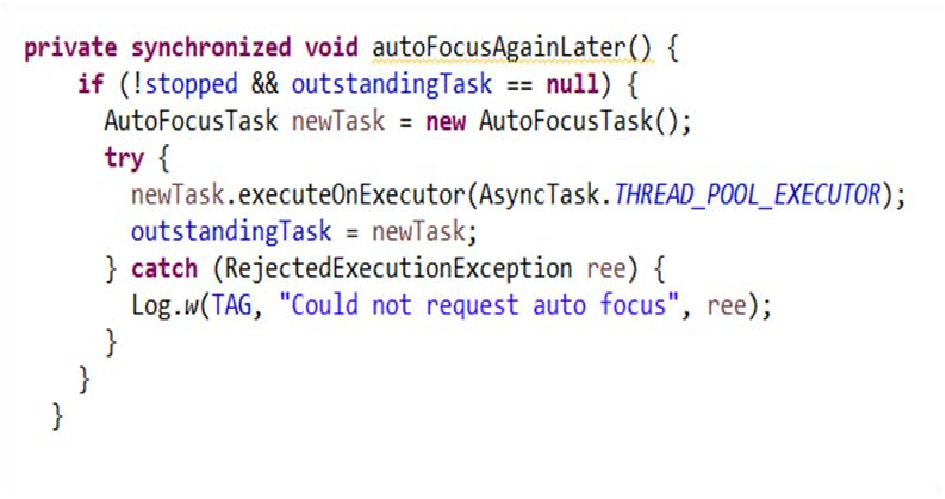
\includegraphics[width=\linewidth]{img/function.pdf}
% \caption{\label{figure:functionExample2}function example}
%\end{figure}

%\begin{figure}[!htp]
% \centering
% 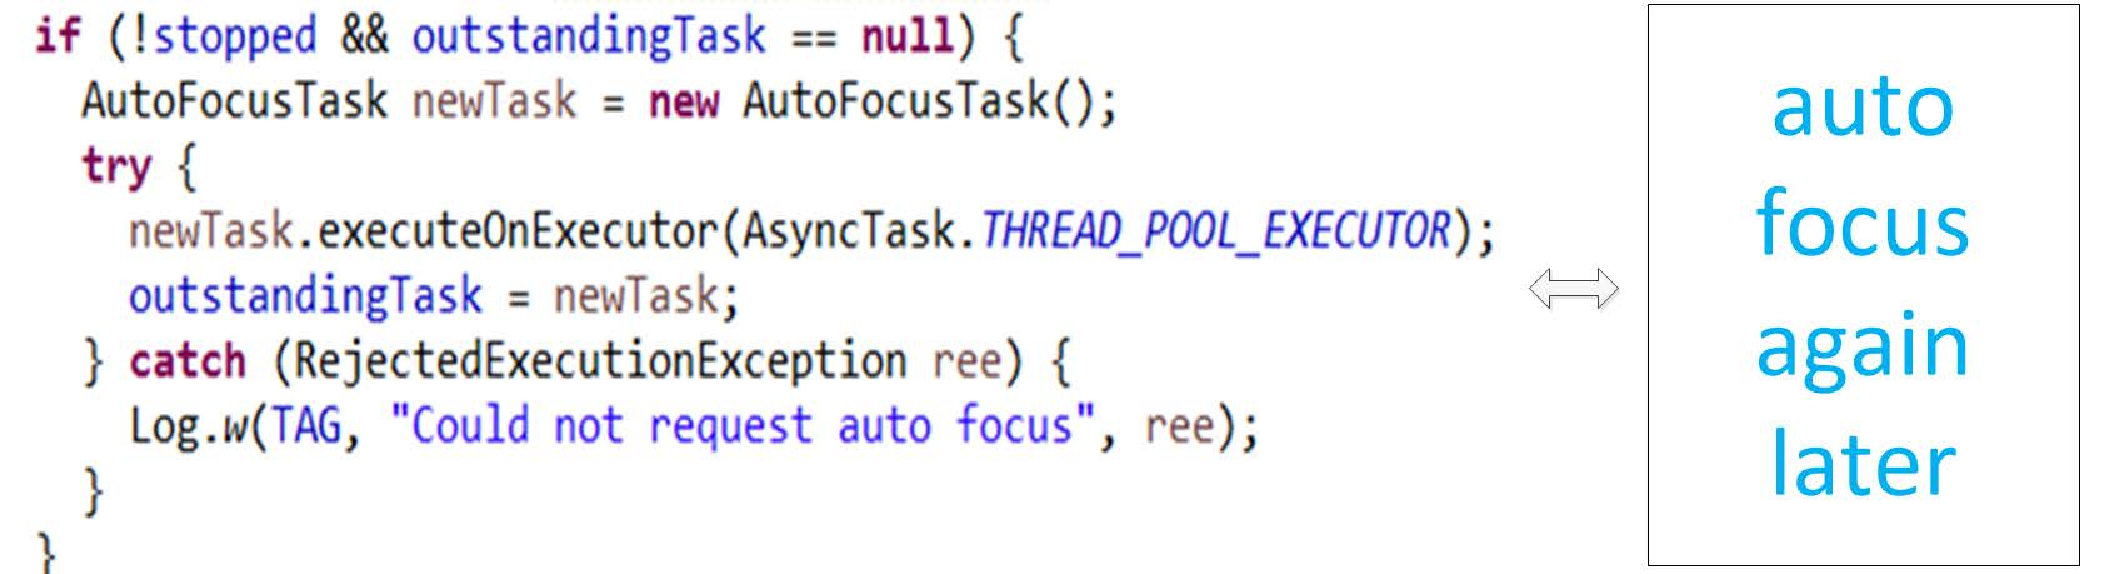
\includegraphics[width=\linewidth]{img/pair.pdf}
% \caption{\label{figure:pairExample} code and tag pair}
%\end{figure}

For evaluation, we choose 100 functions from repository into evaluation data set. Then we sample other 49 function's name as distractor tags for every evaluation function. And because we split all functions' name into individual words, every function may have almost 100 tags as its candidate tags. Our evaluation task is to retrieve the true tags(true tags are split from function's own name) from all candidate tags.
\subsection{Baseline}
To show the effectiveness of our model, we also construct two kinds of baseline. These two baselines are all based on bags of words from source code and don't utilize any structural information such as parse tree and so on.
\subsubsection{TF-IDF}
We firstly extract all identifiers for every function and add them in the vocabulary of repository. For every function, it has own word list, and if one identifier appears in function n times, there will be also n same identifiers in the word list. Then we use TF-IDF approach to compute the relatedness of words to functions. So we can get a vector to represent function and the value of this vector is the TF-IDF value of all words to this function. Meanwhile, we can get a similar vector for every tag that is split from function name. Finally, we calculate the cosine distance between functions and tags. We can rank all candidate tags according to cosine distance for every function.
\subsubsection{Topic Model}\label{sec:topicModel}
In this baseline, we choose the same method to extract the vocabulary and the word list of every function as above. Then we construct a probabilistic model for code repository.
\begin{figure}[!htp]
 \centering
 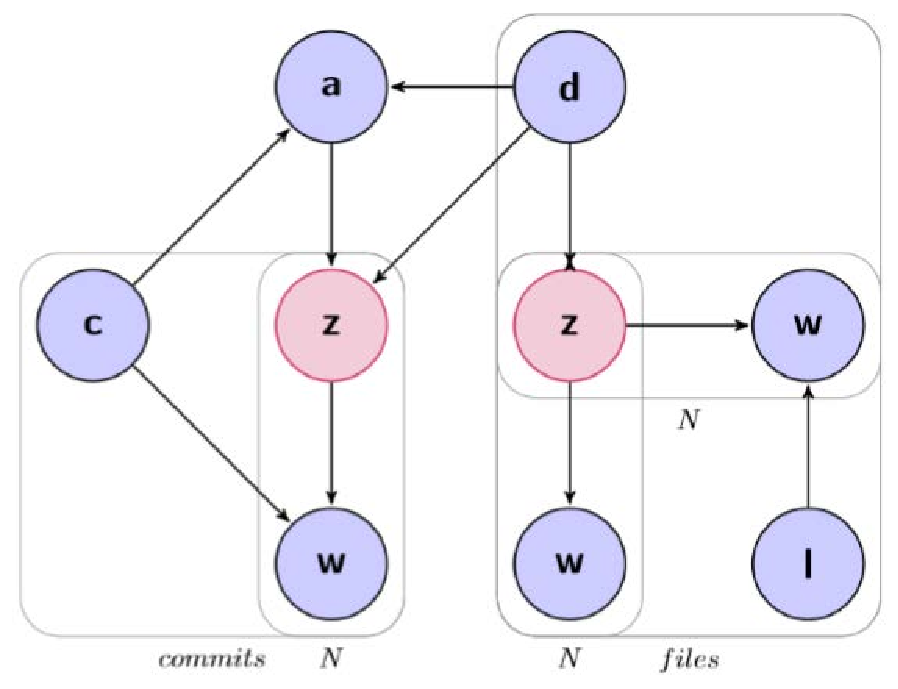
\includegraphics[width=6cm]{img/probabilisticModel.pdf}
 \caption{\label{figure:probModel} probabilistic model}
\end{figure}
As shown in Fig \ref{figure:probModel}, $d$ is the source code function, $z$ is the subject of every function, $w$ is the word that may appear in function $d$, $l$ is the programming language that was used to write this function and c means the comment of function.
Then we can generate one function follows two steps:
\begin{itemize}
    \item generate one subject $z$ follows the multi distribution $multi(z|d)$ with the fixed function $d$.
    \item generate one word that might appear in function $d$ follows the distribution $multi(w|z)$ based on the subject $z$ which was generated just now.
\end{itemize}
When we complete the above two steps, we can generate one word for function $d$. And if we iterate these two steps many times, we can get the whole function $d$.
Next, we decide to use EM algorithm to train our probabilistic model and gain the distribution of $P(z|d)$ and $P(w|z)$. And the equation of calculating probabilistic is:
\begin{align}
    \begin{split}
        P(Data|\phi)=\prod_{m}\prod_{i}(\eta \sum_{k}P(w_{i}|z_{k})P(z_{k}|d_{m})+\\
        (1-\eta)P(w_{i}|s))^{l(w_{i}^{(x)},d_{m})}) \\
        \prod_{j}(\sum_{k}P(w_{j}|z_{k})P(z_{k}|d_{m}))^{l(w_{j}^{(y)},d_{m})}
    \end{split}
\end{align}
where $Data$ is the data of function and $\phi$ is all situations that functions may meet. $l$ is the function that count the time of word $w_{i}$ appears.

Following is the equation of our EM algorithm:
\begin{itemize}
\item E step:
\begin{align}
    P(z_{k}\ |\ w_{i},d_{m}) & = \frac{P(w_{i}\ |\ z_{k})P(z_{k}\ |\ d_{m})}{\sum_{k}P(w_{i}\ |\ z_{k})P(z_{k}\ |\ d_{m})}
\end{align}
\item M step:
\begin{align}
    l(w_{i},d_{m}) = \eta l(w_{i}^{(x)},d_{m})+l(w_{i}^{(y)},d_{m})
\end{align}
 \ To compute $P(w_{i}|z_{k})$
\begin{align}
\begin{split}
    P(w_{i}|z_{k})  =
  \frac{ \sum_{m}\alpha l(w_{i},d_{m})P(z_{k}|w_{i},d_{m})}
  {\sum_{i} \sum_{m} \alpha l(w_{i},d_{m})P(z_{k}|w_{i},d_{m})}\\
  \frac{ +(1-\alpha)l(w_{i},d_{m})\sum_{m^{'}}\beta_{m,m^{'}}P(z_{k}|w_{i},d_{m^{'}})}{ +(1-\alpha)l(w_{i},d_{m})\sum_{m^{'}}\beta_{m,m^{'}}P(z_{k}|w_{i},d_{m^{'}}) }
\end{split}
\end{align}

 \ To compute $P(z_{k}|d_{m})$
\begin{align}
\begin{split}
    P(z_{k}|d_{m})  =
  \frac{ \sum_{i}\alpha l(w_{i},d_{m})P(z_{k}|w_{i},d_{m})}
  {\sum_{k} \sum_{i} \alpha l(w_{i},d_{m})P(z_{k}|w_{i},d_{m})}\\
  \frac{ +(1-\alpha)\sum_{n}l(w_{i},d_{n})\beta_{n,m}P(z_{k}|w_{i},d_{n})}{ +(1-\alpha)\sum_{n}l(w_{i},d_{n})\beta_{n,m}P(z_{k}|w_{i},d_{n}) }
\end{split}
\end{align}

\end{itemize}
\subsection{Result}\label{sec:result}

\subsubsection{Accuracy}
We calculate the accuracy of four model to show our model's effectiveness. And the equation of calculating accuracy is:
\begin{align}
    accuracy & = \frac{\sum_{i=1}^{k}1(pos_{i} \geq n)}{k}
\end{align}
where $pos_{i}$ is the position of $tag_{i}$ in ranked tag list, $n$ is the number of tags that we want to choose and $k$ is the number of tags in groundtruth. The function $1(pos_{i} \geq n)$ means if it is true that $pos_{i} \geq n$ then return 1, else return 0.

For example, we have totaly 10 tags in the list and 2 tags $tag_{1}$ and $tag_{2}$ in groundtruth. The position of $tag_{1}$ and $tag_{2}$ are second and seventh position respectively. If we only choose 5 tags from tag list, the accuracy will be 0.5 ($\frac{1+0}{2}=0.5$).

Fig \ref{figure:accuracyOfFour} shows the result of four model when we choose 5 and 10 tags from almost 100 tags. We can see that there are four histograms that represent the accuracy of four models respectively.
%four different color lines for different number of tags. The red line is the accuracy of our model, green one is the result of Miltiadis's model, the blue line shows the accuracy of our topic model baseline and finally the black line is the accuracy of TF-IDF model. The different color rectangle measures the approvement between this model and the previous one. For example, the red rectangle measures the increase between our model and Miltiadis's model. The larger the area, the greater the increase.
From Fig \ref{figure:accuracyOfFour} we can know our model is the best one and the improvement between Allamanis et al's model and topic model is the largest one.

Fig \ref{figure:accuracyOfDiffTags} shows the accuracy of our model and Allamanis et al's model when we choose tags from one to fifty. We can see our model is always better than Allamanis et al's model. And when we choose 50 tags, accuracy is almost 0.9, so we can say that most of our tags are at the first half position(every function has 100 candidate tags).
\begin{figure}[!htp]
 \centering
 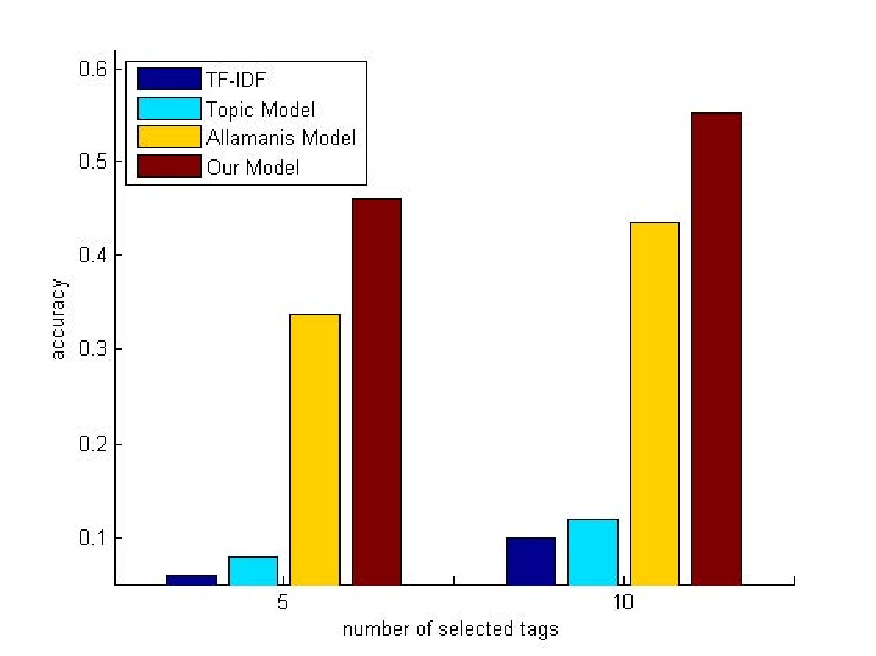
\includegraphics[width=\linewidth]{img/accuracy1.pdf}
 \caption{\label{figure:accuracyOfFour} accuracy of four model}
\end{figure}

\begin{figure}[!htp]
 \centering
 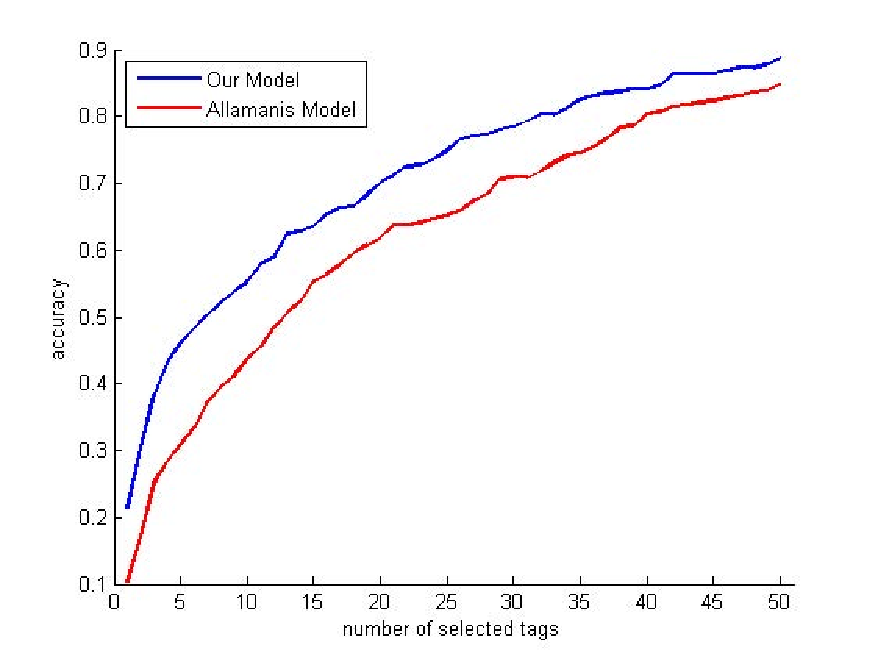
\includegraphics[width=\linewidth]{img/accuracy2.pdf}
 \caption{\label{figure:accuracyOfDiffTags} accuracy of different number of tags}
\end{figure}

\subsubsection{MRR}
We also use MRR(Mean reciprocal rank) to evaluate our model. When we calculate MRR, we firstly get tags that from the same function name together as a group and rank them with other groups. For example, if there are tow functions whose names are readBuffer and getNumber. We can get four tags read, buffer, get and number. And we make read and buffer are in one group and get and number are in one group. So our result of ranking is the first one is read and buffer, the second one is get and number. By the way, because of group, number of candidates becomes 50 for every function.

Fig \ref{figure:resultMRR} shows the MRR of 10 different source code repositories. The source code of these repositories are all downloaded from github directly. We see that our model's average MRR are all better than Allamanis et al's model on 10 repositories, and on some repositories our result is double of Allamanis et al's model.
\begin{figure}[!htp]
 \centering
 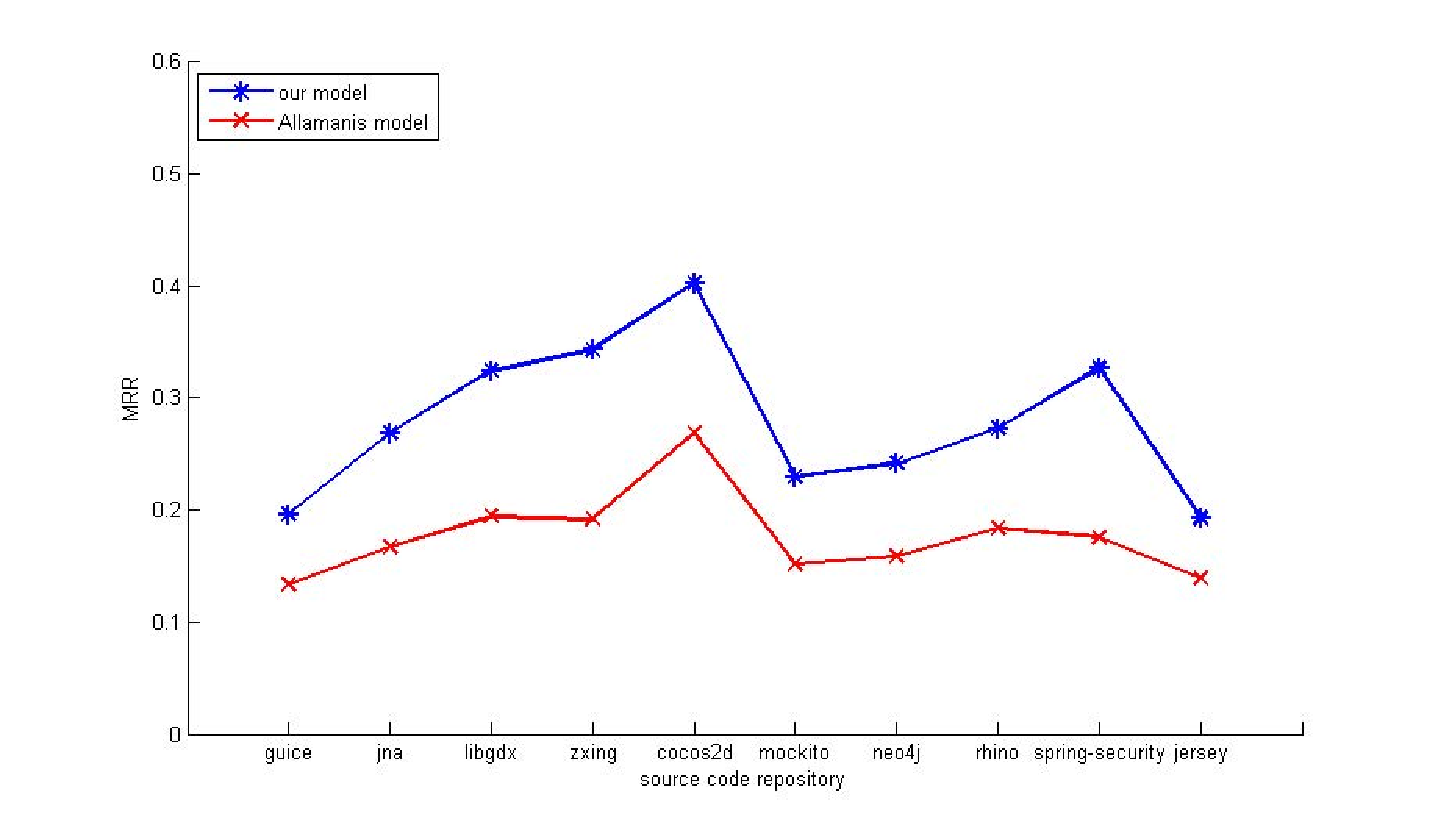
\includegraphics[width=\linewidth]{img/MRR.pdf}
 \caption{\label{figure:resultMRR} result of MRR}
\end{figure}

\subsubsection{With or without comments}
Because comments in the source code often contain much information of source codes's function, we also want to add the comments into our model. The different results of with or without comments model are shown in Fig \ref{figure:MRRComments}. From Fig \ref{figure:MRRComments}, we know that the MRR isn't always become better after adding comments information but it is close to original results at least.

So wether comments is useful is based on the quality of comments. If comments contains much meaningful information of function, the result will be better with comments. On the contrary, if the quality of comments is bad and most of comments are source code that were given up by programmer, the result won't be improved or even become a little worse. Source code repository guice's comments are an example of bad comments. Guice's comments can't help to gain the function of method. And zxing's comments is the good example of comments, these comments help model to extract much more meaningful information about the function of methods. Some examples about good and bad comments are shown in Table \ref{table:comments}. We can see that the comments from guice repository only tell us human can see some examples at which place but don't tell us any information about function of method, so this kind comment won't improve the performance of our model.
\begin{figure}[!htp]
 \centering
 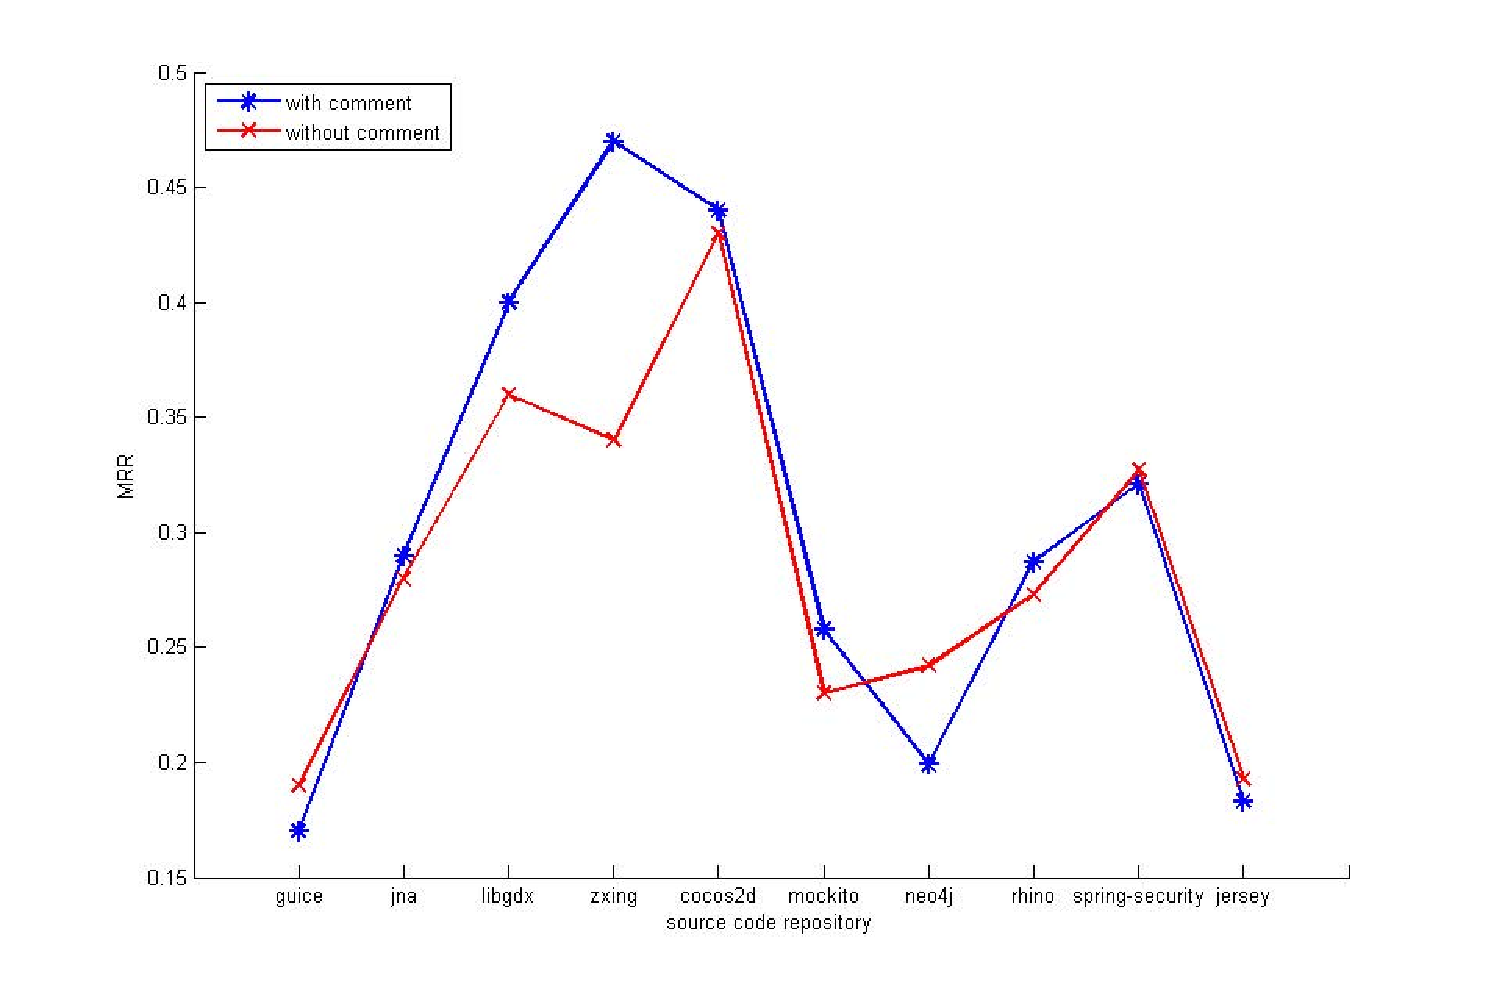
\includegraphics[width=\linewidth]{img/CompareComment.pdf}
 \caption{\label{figure:MRRComments} MRR of with/without comments}
\end{figure}

\begin{table*}[!htp]
\centering
\caption{ \label{table:comments} Example of good and bad comments}
\begin{tabular}{|p{10cm}|p{3cm}|p{3cm}|}
\hline
Example & Good or Bad & Source file\\
\hline
 & & \\
public interface OverriddenModuleBuilder \{ & &\\

\textcolor[rgb]{0,0,1}{
    /** }& & \\
\textcolor[rgb]{0,0,1}{     * See the EDSL example at \{@link Modules\#override(Module[]) override()\}. }& & \\
 \textcolor[rgb]{0,0,1}{    */}& & \\
    Module with(Module... overrides);& & \\

\textcolor[rgb]{0,0,1}{
    /**}& Bad & guice/core/src/com/google/ \\
\textcolor[rgb]{0,0,1}{     * See the EDSL example at \{@link Modules\#override(Module[]) override()\}.}& & inject/util/Modules.java  \\
\textcolor[rgb]{0,0,1}{     */}& & \\

    Module with(Iterable$<?$ extends Module$>$ overrides); & & \\

  \}
 &  & \\

  & & \\

\hline
 & & \\
public boolean isRange(int start, int end, boolean value) \{ & & \\
    if (end $<$ start) \{ & & \\
      throw new IllegalArgumentException(); & & \\
    \} & & \\
    if (end == start) \{ & & \\
      return true; \textcolor[rgb]{0,0,1}{ // empty range matches }& & \\
    \} & & \\
    end--; \textcolor[rgb]{0,0,1}{ // will be easier to treat this as the last actually set bit -- inclusive} & & \\
    int firstInt = start / 32; & & \\
    int lastInt = end / 32; & & \\
    for (int i = firstInt; i $<=$ lastInt; i++) \{ & & \\
      int firstBit = i $>$ firstInt ? 0 : start \& 0x1F; & & \\
      int lastBit = i $<$ lastInt ? 31 : end \& 0x1F; & &  \\
      int mask; & & zxing/core/src/main/java/ \\
      if (firstBit == 0 \&\& lastBit == 31) \{ & Good & com/google/zxing/common/ \\
        mask = -1; & & BitArray.java \\
      \} else \{ & & \\
        mask = 0; & & \\
        for (int j = firstBit; j $<=$ lastBit; j++) \{ & & \\
          mask $|$= 1 $<<$ j; & & \\
        \} & & \\
      \} & & \\

\textcolor[rgb]{0,0,1}{
      // Return false if we're looking for 1s and the masked bits[i] isn't all 1s (that is,} & & \\
\textcolor[rgb]{0,0,1}{      // equals the mask, or we're looking for 0s and the masked portion is not all 0s} & & \\
      if ((bits[i] \& mask) != (value ? mask : 0)) \{ & & \\
        return false; & & \\
      \} & & \\
    \} & &  \\
    return true; & & \\
  \}
 &  & \\
  & & \\
\hline
 & & \\
\textcolor[rgb]{0,0,1}{
/** Reduces the size of the array to the specified size. If the array is already smaller than the specified size, no action is} & & \\
     \textcolor[rgb]{0,0,1}{    * taken. */} & & \\
        public void truncate (int newSize) \{ & & cocos2d/cocos2d-android/ \\
                if (size $<$= newSize) return; & Good & src/com/badlogic/ \\
                for (int i = newSize; i $<$ size; i++) & & gdx/utils/Array.java \\
                        items[i] = null; & &  \\
                size = newSize; & &  \\
        \} &  & \\
& & \\
\hline
\end{tabular}

\end{table*}

\subsubsection{Example of MRR Result}
There is one output example of our model and Miltiadis's model in Table \ref{table:MRRExample}. From Table \ref{table:MRRExample} we can see that the target tags are at the second position in our model and the first one is set. The tag "set" is related to the subject of function setRelativeAnchorPoint, so put it as the first one is reasonable. But the result of Miltiadis's model is much worse, the groundtruth is at the fifth position and the first recommended tag is "set center". Obviously, the word "center" isn't related to subject. And we only put the top 10 recommended tags in the table. The third function in table is too long, we only put part of them and the results of two models are same, first position. Due to the result of Miltiadi's model for the forth function, there are no true tags in the top 10 recommended tags while true tag is at forth position in our model.
\begin{table*}[!htbp]
    \centering
    \caption{\label{table:MRRExample} Example of the result to calculate MRR  }
    \begin{tabular} {|p{10cm}|p{3cm}|p{3cm}|}
    \hline
    Function & our model result & Miltiadis's model\\
    \hline
    & & \\
    & set & set center\\
    & \textbf{set relative anchor point} & get motor torque \\
    Public void setRelativeAnchorPoint(Boolean newValue) \{ &get radius & table cell at index\\
    \  \ \  \  isRelativeAnchorPoint = newValue; & get body count & get next\\
    \  \ \  \  isTransformDirty\_ = isInverseDirty+ = true;  & get device orientation & \textbf{set relative anchor point} \\
	\  \ \  \ if (ccConfig.CC\_NODE\_TRANSFORM\_USING\_AFFINE\_MATRIX) \{ & get next & conver to ui\\
	\  \ \  \ \  \ \  \ \	isTransformGLDirty\_ = true;  & get world center & set angle \\
	\  \ \  \  \}   &  get translation & set texture \\
    \} & get texture rect rotated & get texture \\
    & set cqpoint & set limits \\
    & & \\
    \hline

    & & \\
& \textbf{get color} & set \\
& get value & \textbf{get color}\\
& get blend func & get center \\
& get rotation & get action \\
    public ccColor3B getColor()\{ & tile & get restitution \\
    \  \ \  \ return ccColor3B.ccc3(color\_\.r, color\_\.g, color\_\.b); & get tangent normals & get target \\
    \} & get tex env param& get joint list \\
& set length & get normals \\
& set texture & get world vector\\
& action & get priority\\

    & & \\
    \hline

    & & \\

    private long createProperJoint(JointDef def) \{ & \textbf{create proper joint}& \textbf{create proper joint} \\
  \  \ \  \  if (def.type == JointType.DistanceJoint) \{ & get next & get\\
  \  \ \  \ \  \ \  \  DistanceJointDef d = (DistanceJointDef) def; & get damping ratio & set position \\
  \  \ \  \ \  \ \  \ \  return jniCreateDistanceJoint(addr,d.bodyA.addr,d.bodyB.addr,d.collideConnected, & convert to world space & set opacity modify rgb\\
  \  \ \  \ \  \ \  \  \  \ \  \ d.localAnchorA.x,d.localAnchorA.y,d.localAnchorB.x,d.localAnchorB.y & get world manifold & get x \\
  \  \ \  \ \  \ \  \ \  \ \  \   ,d.length,d.frequencyHz,d.dampingRatio);  & get density & set color\\
    & to double pow & get running scene\\
  \  \ \  \  \} & get contact register & get percentage \\

  \  \ \  \ \  \ \  \   \textbf{...} & get centroid & set radial accel \\
  \  \ \  \ \  \ \  \   \textbf{...} & is running& set blend func\\
  \  \ \  \ \  \ \  \    & & \\

  \  \ \  \   if (def.type == JointType.WheelJoint) \{ & & \\
  \  \ \  \ \  \ \  \   WheelJointDef d = (WheelJointDef) def; & & \\
  \  \ \  \ \  \ \  \   return jniCreateDistanceJoint(addr,d.bodyA.addr,d.bodyB.addr,d.collideConnected, & & \\
  \  \ \  \ \  \ \  \   \  \ \  \ d.localAnchorA.x,d.localAnchorA.y,d.localAnchorB.x,d.localAnchorB.y & & \\
  \  \ \  \ \  \ \  \  \  \ \  \ ,d.localAxisA.x,d.enableMotor,d.maxMotroTorque, d.motorSpeed,    & & \\
  \  \ \  \ \  \ \ \  \ \  \ \ d.frequencyHz,d.dampingRatio);  & & \\
  \  \ \  \   \} & & \\

  \  \ \  \   return 0; & & \\
    \} & & \\
    & & \\
    \hline

    & & \\
    & get body & set motor speed \\
& get text coords & set y \\
& get blend func & set tile \\
& \textbf{get max density}& get next \\
    public double getMaxDensity() \{ & get position & get aabb \\
  \  \ \  \   return maxDensity; & get scale& get joints \\
    \} & set opacity & set to ortho \\
& get tex env param & set priority \\
& get tangent normals & get color \\
& set to translation & is motor enabled \\

    & & \\
    \hline

    & & \\
    & gl get integerv & set string \\
& add motion listener & on destroy \\
& \textbf{post step} & set visible \\
    private void postStep(float dt, int iterations) \{  & on resume & fill float buffer \\
  \  \ \  \   for (Steppable s:postStepList) \{ & draw string & set blend func \\
  \  \ \  \ \  \ \  \   s.step(dt,iterations); & set original target & \textbf{post step}\\
  \  \ \  \   \} & draw & set label \\
    \} & next callback& node \\
& add point & position for ortho at \\
& get anchor & set grid size \\

    & & \\
    \hline
    \end{tabular}
\end{table*}
